\section{Auswertung}
\label{sec:Auswertung}
\subsection{Winkelrichtgröße}
Die Winkelrichtgröße wird durch die Formel
\begin{equation}
  D = \frac{F \cdot r}{\phi}
\end{equation}
bestimmt. Die verwendeten Werte sind in \ref{tab:winkelrichtgr} angegeben.
\begin{table}
  \centering
  \label{tab:winkelrichtgr}
  \caption{Messdaten zur Bestimmung der Winkelrichtgröße D}
  \begin{tabular}{c c c c}
    \toprule
    $F/N$ & $\phi$ & $r/m$ & $D/Nm$ \\
    \midrule
    0,1  &  30 & 0,1 & 0,000333\\
    0,26 &  60 & 0,1 & 0,000433\\
    0,41 &  90 & 0,1 & 0,000456\\
    0,56 & 120 & 0,1 & 0,000467\\
    0,72 & 150 & 0,1 & 0,000480\\
    0,85 & 180 & 0,1 & 0,000472\\
    0,48 & 180 & 0,2 & 0,000533\\
    0,55 & 240 & 0,2 & 0,000458\\
    0,63 & 270 & 0,2 & 0,000467\\
    0,69 & 300 & 0,2 & 0,000460\\
    \bottomrule
  \end{tabular}
\end{table}
\\Sowohl der Mittelwert, als auch die Standardabweichung wurden mit Python bestimmt. Daraus ergibt sich der
gemittelte Wert
\begin{align*}
    D = (0.000456 \pm 0{,}000048)\,\mathrm{Nm} .
\end{align*}

\subsection{Eigenträgheitsmoment}
\begin{figure}
  \centering
  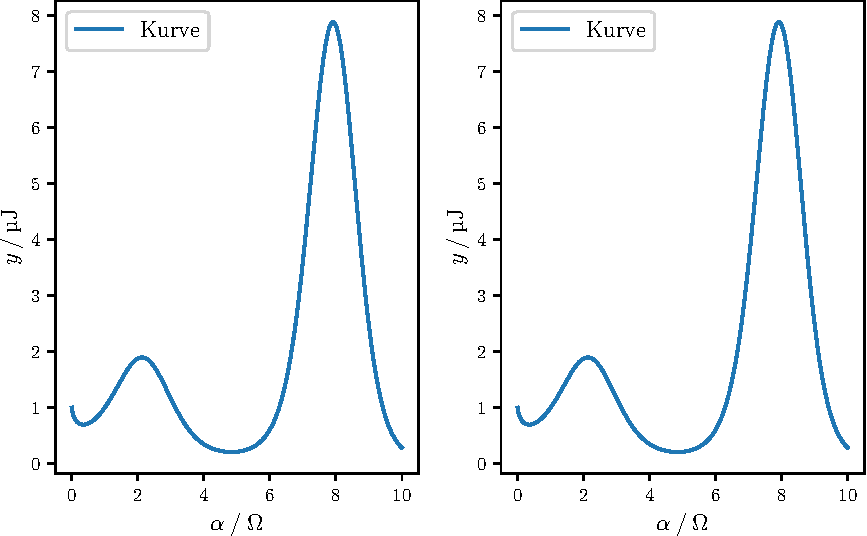
\includegraphics{plot.pdf}
  \caption{Plot.}
  \label{fig:plot}
\end{figure}

\subsection{Trägheitsmoment des Zylinders}
\subsubsection{Theoretische Werte}
\subsubsection{Experimentelle Werte}
\subsection{Trägheitsmoment der Kugel}
\subsubsection{Theoretische Werte}
\subsubsection{Experimentelle Werte}


Siehe \autoref{fig:plot}!
